\documentclass[twoside]{book}

% Packages required by doxygen
\usepackage{fixltx2e}
\usepackage{calc}
\usepackage{doxygen}
\usepackage[export]{adjustbox} % also loads graphicx
\usepackage{graphicx}
\usepackage[utf8]{inputenc}
\usepackage{makeidx}
\usepackage{multicol}
\usepackage{multirow}
\PassOptionsToPackage{warn}{textcomp}
\usepackage{textcomp}
\usepackage[nointegrals]{wasysym}
\usepackage[table]{xcolor}

% Font selection
\usepackage[T1]{fontenc}
\usepackage[scaled=.90]{helvet}
\usepackage{courier}
\usepackage{amssymb}
\usepackage{sectsty}
\renewcommand{\familydefault}{\sfdefault}
\allsectionsfont{%
  \fontseries{bc}\selectfont%
  \color{darkgray}%
}
\renewcommand{\DoxyLabelFont}{%
  \fontseries{bc}\selectfont%
  \color{darkgray}%
}
\newcommand{\+}{\discretionary{\mbox{\scriptsize$\hookleftarrow$}}{}{}}

% Page & text layout
\usepackage{geometry}
\geometry{%
  a4paper,%
  top=2.5cm,%
  bottom=2.5cm,%
  left=2.5cm,%
  right=2.5cm%
}
\tolerance=750
\hfuzz=15pt
\hbadness=750
\setlength{\emergencystretch}{15pt}
\setlength{\parindent}{0cm}
\setlength{\parskip}{3ex plus 2ex minus 2ex}
\makeatletter
\renewcommand{\paragraph}{%
  \@startsection{paragraph}{4}{0ex}{-1.0ex}{1.0ex}{%
    \normalfont\normalsize\bfseries\SS@parafont%
  }%
}
\renewcommand{\subparagraph}{%
  \@startsection{subparagraph}{5}{0ex}{-1.0ex}{1.0ex}{%
    \normalfont\normalsize\bfseries\SS@subparafont%
  }%
}
\makeatother

% Headers & footers
\usepackage{fancyhdr}
\pagestyle{fancyplain}
\fancyhead[LE]{\fancyplain{}{\bfseries\thepage}}
\fancyhead[CE]{\fancyplain{}{}}
\fancyhead[RE]{\fancyplain{}{\bfseries\leftmark}}
\fancyhead[LO]{\fancyplain{}{\bfseries\rightmark}}
\fancyhead[CO]{\fancyplain{}{}}
\fancyhead[RO]{\fancyplain{}{\bfseries\thepage}}
\fancyfoot[LE]{\fancyplain{}{}}
\fancyfoot[CE]{\fancyplain{}{}}
\fancyfoot[RE]{\fancyplain{}{\bfseries\scriptsize Generated by Doxygen }}
\fancyfoot[LO]{\fancyplain{}{\bfseries\scriptsize Generated by Doxygen }}
\fancyfoot[CO]{\fancyplain{}{}}
\fancyfoot[RO]{\fancyplain{}{}}
\renewcommand{\footrulewidth}{0.4pt}
\renewcommand{\chaptermark}[1]{%
  \markboth{#1}{}%
}
\renewcommand{\sectionmark}[1]{%
  \markright{\thesection\ #1}%
}

% Indices & bibliography
\usepackage{natbib}
\usepackage[titles]{tocloft}
\setcounter{tocdepth}{3}
\setcounter{secnumdepth}{5}
\makeindex

% Hyperlinks (required, but should be loaded last)
\usepackage{ifpdf}
\ifpdf
  \usepackage[pdftex,pagebackref=true]{hyperref}
\else
  \usepackage[ps2pdf,pagebackref=true]{hyperref}
\fi
\hypersetup{%
  colorlinks=true,%
  linkcolor=blue,%
  citecolor=blue,%
  unicode%
}

% Custom commands
\newcommand{\clearemptydoublepage}{%
  \newpage{\pagestyle{empty}\cleardoublepage}%
}

\usepackage{caption}
\captionsetup{labelsep=space,justification=centering,font={bf},singlelinecheck=off,skip=4pt,position=top}

%===== C O N T E N T S =====

\begin{document}

% Titlepage & ToC
\hypersetup{pageanchor=false,
             bookmarksnumbered=true,
             pdfencoding=unicode
            }
\pagenumbering{roman}
\begin{titlepage}
\vspace*{7cm}
\begin{center}%
{\Large My Project }\\
\vspace*{1cm}
{\large Generated by Doxygen 1.8.11}\\
\end{center}
\end{titlepage}
\clearemptydoublepage
\tableofcontents
\clearemptydoublepage
\pagenumbering{arabic}
\hypersetup{pageanchor=true}

%--- Begin generated contents ---
\chapter{Hierarchical Index}
\section{Class Hierarchy}
This inheritance list is sorted roughly, but not completely, alphabetically\+:\begin{DoxyCompactList}
\item \contentsline{section}{Fruit}{\pageref{classFruit}}{}
\begin{DoxyCompactList}
\item \contentsline{section}{Apple}{\pageref{classApple}}{}
\item \contentsline{section}{Grape}{\pageref{classGrape}}{}
\item \contentsline{section}{Orange}{\pageref{classOrange}}{}
\end{DoxyCompactList}
\item \contentsline{section}{List}{\pageref{classList}}{}
\item \contentsline{section}{List\+:\+:Node}{\pageref{structList_1_1Node}}{}
\end{DoxyCompactList}

\chapter{Class Index}
\section{Class List}
Here are the classes, structs, unions and interfaces with brief descriptions\+:\begin{DoxyCompactList}
\item\contentsline{section}{\hyperlink{structnode}{node} }{\pageref{structnode}}{}
\item\contentsline{section}{\hyperlink{structnode1}{node1} }{\pageref{structnode1}}{}
\item\contentsline{section}{\hyperlink{structnode__info}{node\+\_\+info} }{\pageref{structnode__info}}{}
\end{DoxyCompactList}

\chapter{File Index}
\section{File List}
Here is a list of all files with brief descriptions\+:\begin{DoxyCompactList}
\item\contentsline{section}{\hyperlink{Lab1_8c}{Lab1.\+c} }{\pageref{Lab1_8c}}{}
\end{DoxyCompactList}

\chapter{Class Documentation}
\hypertarget{classAnimal}{}\section{Animal Class Reference}
\label{classAnimal}\index{Animal@{Animal}}


Inheritance diagram for Animal\+:
\nopagebreak
\begin{figure}[H]
\begin{center}
\leavevmode
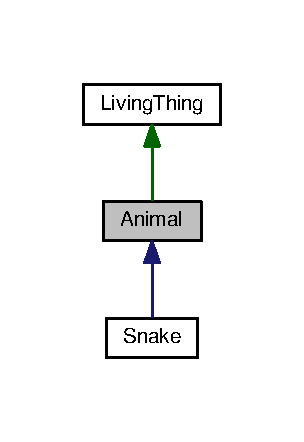
\includegraphics[width=146pt]{classAnimal__inherit__graph}
\end{center}
\end{figure}


Collaboration diagram for Animal\+:
\nopagebreak
\begin{figure}[H]
\begin{center}
\leavevmode
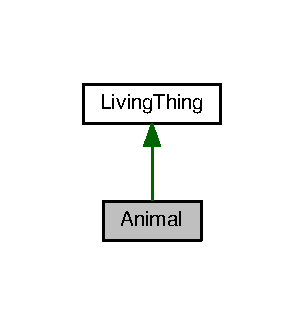
\includegraphics[width=146pt]{classAnimal__coll__graph}
\end{center}
\end{figure}
\subsection*{Protected Member Functions}
\begin{DoxyCompactItemize}
\item 
void \hyperlink{classAnimal_aa42d90cae6c72833565ed1af72585bad}{breathe} ()
\end{DoxyCompactItemize}


\subsection{Member Function Documentation}
\index{Animal@{Animal}!breathe@{breathe}}
\index{breathe@{breathe}!Animal@{Animal}}
\subsubsection[{\texorpdfstring{breathe()}{breathe()}}]{\setlength{\rightskip}{0pt plus 5cm}void Animal\+::breathe (
\begin{DoxyParamCaption}
{}
\end{DoxyParamCaption}
)\hspace{0.3cm}{\ttfamily [inline]}, {\ttfamily [protected]}}\hypertarget{classAnimal_aa42d90cae6c72833565ed1af72585bad}{}\label{classAnimal_aa42d90cae6c72833565ed1af72585bad}

\begin{DoxyCode}
12                    \{
13         std::cout << \textcolor{stringliteral}{"I'm breathing as an animal."} << std::endl;
14     \}
\end{DoxyCode}


The documentation for this class was generated from the following file\+:\begin{DoxyCompactItemize}
\item 
\hyperlink{DiamondProblem_8cpp}{Diamond\+Problem.\+cpp}\end{DoxyCompactItemize}

\hypertarget{classLivingThing}{}\section{Living\+Thing Class Reference}
\label{classLivingThing}\index{Living\+Thing@{Living\+Thing}}


Inheritance diagram for Living\+Thing\+:
\nopagebreak
\begin{figure}[H]
\begin{center}
\leavevmode
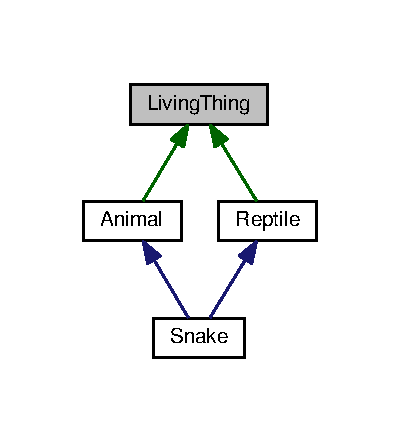
\includegraphics[width=192pt]{classLivingThing__inherit__graph}
\end{center}
\end{figure}
\subsection*{Protected Member Functions}
\begin{DoxyCompactItemize}
\item 
void \hyperlink{classLivingThing_a6b97287cf8d8ef975f05f08b82a023bf}{breathe} ()
\end{DoxyCompactItemize}


\subsection{Member Function Documentation}
\index{Living\+Thing@{Living\+Thing}!breathe@{breathe}}
\index{breathe@{breathe}!Living\+Thing@{Living\+Thing}}
\subsubsection[{\texorpdfstring{breathe()}{breathe()}}]{\setlength{\rightskip}{0pt plus 5cm}void Living\+Thing\+::breathe (
\begin{DoxyParamCaption}
{}
\end{DoxyParamCaption}
)\hspace{0.3cm}{\ttfamily [inline]}, {\ttfamily [protected]}}\hypertarget{classLivingThing_a6b97287cf8d8ef975f05f08b82a023bf}{}\label{classLivingThing_a6b97287cf8d8ef975f05f08b82a023bf}

\begin{DoxyCode}
5                    \{
6         std::cout << \textcolor{stringliteral}{"I'm breathing as a living thing."} << std::endl;
7     \}
\end{DoxyCode}


The documentation for this class was generated from the following file\+:\begin{DoxyCompactItemize}
\item 
\hyperlink{DiamondProblem_8cpp}{Diamond\+Problem.\+cpp}\end{DoxyCompactItemize}

\hypertarget{classReptile}{}\section{Reptile Class Reference}
\label{classReptile}\index{Reptile@{Reptile}}


Inheritance diagram for Reptile\+:
\nopagebreak
\begin{figure}[H]
\begin{center}
\leavevmode
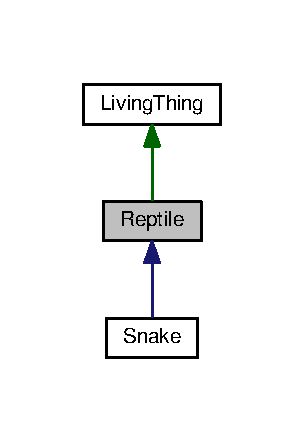
\includegraphics[width=146pt]{classReptile__inherit__graph}
\end{center}
\end{figure}


Collaboration diagram for Reptile\+:
\nopagebreak
\begin{figure}[H]
\begin{center}
\leavevmode
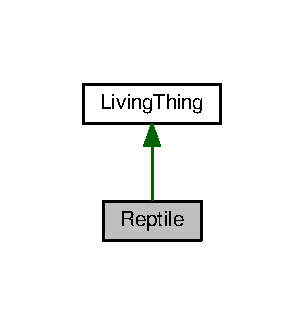
\includegraphics[width=146pt]{classReptile__coll__graph}
\end{center}
\end{figure}
\subsection*{Public Member Functions}
\begin{DoxyCompactItemize}
\item 
void \hyperlink{classReptile_a7131e0e3fe121e20e3a37345ebeb6781}{crawl} ()
\end{DoxyCompactItemize}
\subsection*{Additional Inherited Members}


\subsection{Member Function Documentation}
\index{Reptile@{Reptile}!crawl@{crawl}}
\index{crawl@{crawl}!Reptile@{Reptile}}
\subsubsection[{\texorpdfstring{crawl()}{crawl()}}]{\setlength{\rightskip}{0pt plus 5cm}void Reptile\+::crawl (
\begin{DoxyParamCaption}
{}
\end{DoxyParamCaption}
)\hspace{0.3cm}{\ttfamily [inline]}}\hypertarget{classReptile_a7131e0e3fe121e20e3a37345ebeb6781}{}\label{classReptile_a7131e0e3fe121e20e3a37345ebeb6781}

\begin{DoxyCode}
19                  \{
20         std::cout << \textcolor{stringliteral}{"I'm crawling as a reptile."} << std::endl;
21     \}
\end{DoxyCode}


The documentation for this class was generated from the following file\+:\begin{DoxyCompactItemize}
\item 
\hyperlink{DiamondProblem_8cpp}{Diamond\+Problem.\+cpp}\end{DoxyCompactItemize}

\hypertarget{classSnake}{}\section{Snake Class Reference}
\label{classSnake}\index{Snake@{Snake}}


Inheritance diagram for Snake\+:
\nopagebreak
\begin{figure}[H]
\begin{center}
\leavevmode
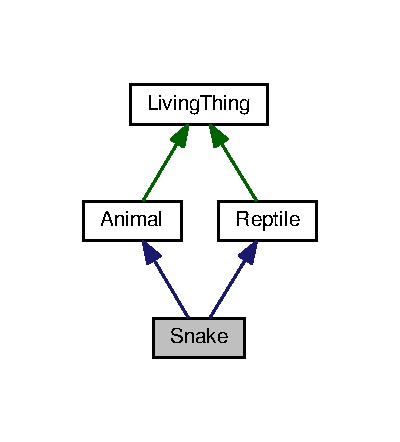
\includegraphics[width=192pt]{classSnake__inherit__graph}
\end{center}
\end{figure}


Collaboration diagram for Snake\+:
\nopagebreak
\begin{figure}[H]
\begin{center}
\leavevmode
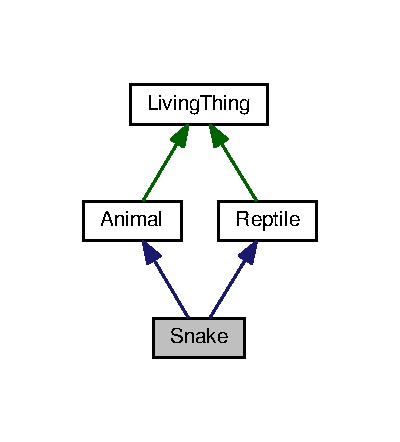
\includegraphics[width=192pt]{classSnake__coll__graph}
\end{center}
\end{figure}
\subsection*{Additional Inherited Members}


The documentation for this class was generated from the following file\+:\begin{DoxyCompactItemize}
\item 
\hyperlink{DiamondProblem_8cpp}{Diamond\+Problem.\+cpp}\end{DoxyCompactItemize}

\chapter{File Documentation}
\hypertarget{DiamondProblem_8cpp}{}\section{Diamond\+Problem.\+cpp File Reference}
\label{DiamondProblem_8cpp}\index{Diamond\+Problem.\+cpp@{Diamond\+Problem.\+cpp}}
{\ttfamily \#include $<$iostream$>$}\\*
Include dependency graph for Diamond\+Problem.\+cpp\+:
\nopagebreak
\begin{figure}[H]
\begin{center}
\leavevmode
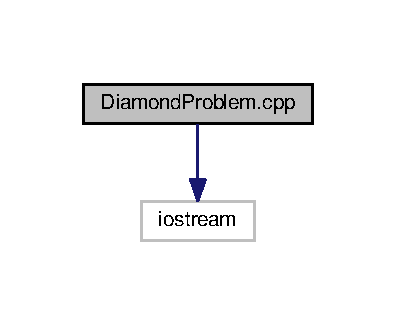
\includegraphics[width=190pt]{DiamondProblem_8cpp__incl}
\end{center}
\end{figure}
\subsection*{Classes}
\begin{DoxyCompactItemize}
\item 
class \hyperlink{classLivingThing}{Living\+Thing}
\item 
class \hyperlink{classAnimal}{Animal}
\item 
class \hyperlink{classReptile}{Reptile}
\item 
class \hyperlink{classSnake}{Snake}
\end{DoxyCompactItemize}
\subsection*{Functions}
\begin{DoxyCompactItemize}
\item 
int \hyperlink{DiamondProblem_8cpp_ae66f6b31b5ad750f1fe042a706a4e3d4}{main} ()
\end{DoxyCompactItemize}


\subsection{Function Documentation}
\index{Diamond\+Problem.\+cpp@{Diamond\+Problem.\+cpp}!main@{main}}
\index{main@{main}!Diamond\+Problem.\+cpp@{Diamond\+Problem.\+cpp}}
\subsubsection[{\texorpdfstring{main()}{main()}}]{\setlength{\rightskip}{0pt plus 5cm}int main (
\begin{DoxyParamCaption}
{}
\end{DoxyParamCaption}
)}\hypertarget{DiamondProblem_8cpp_ae66f6b31b5ad750f1fe042a706a4e3d4}{}\label{DiamondProblem_8cpp_ae66f6b31b5ad750f1fe042a706a4e3d4}

\begin{DoxyCode}
28            \{
29     \hyperlink{classSnake}{Snake} snake;
30 
31     snake.\hyperlink{classAnimal_aa42d90cae6c72833565ed1af72585bad}{breathe}();
32     snake.\hyperlink{classReptile_a7131e0e3fe121e20e3a37345ebeb6781}{crawl}();
33 
34     \textcolor{keywordflow}{return} 0;
35 \}\end{DoxyCode}


Here is the call graph for this function\+:
\nopagebreak
\begin{figure}[H]
\begin{center}
\leavevmode
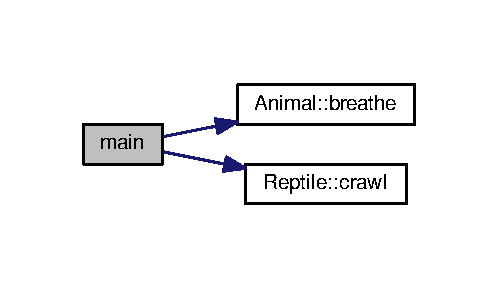
\includegraphics[width=239pt]{DiamondProblem_8cpp_ae66f6b31b5ad750f1fe042a706a4e3d4_cgraph}
\end{center}
\end{figure}



%--- End generated contents ---

% Index
\backmatter
\newpage
\phantomsection
\clearemptydoublepage
\addcontentsline{toc}{chapter}{Index}
\printindex

\end{document}
